\documentclass{IOS-Book-Article}

% gb4e is buggy
\makeatletter
\def\new@fontshape{}
\makeatother

\usepackage[utf8]{inputenc}
\usepackage{amsmath}
\usepackage{amssymb}
\usepackage{amsthm}
\usepackage{mathptmx}
% \usepackage{caption} % for \figsentence
\usepackage{subcaption} % for subfigure
\usepackage{graphicx}
\usepackage{tikz}
\usepackage{tikz-qtree}
\usepackage{syntax} % for grammar environment
\usetikzlibrary{arrows.meta,positioning,patterns}
\usepackage{hyperref} % for urls
\usepackage{gb4e}

\newcommand{\figsentence}[1]{\\{\sffamily{}#1}}

\tikzset{
	x/.style={{Rays[]}},
	-x/.style={-{Rays[]}},
	xx/.style={Rays[]}-{Rays[]},
	box/.style={draw,rectangle,align=center},
	assumed/.style={pattern=crosshatch dots,pattern color=gray},
	every new ->/.style={shorten >=1pt}
}

\begin{document}

	\begin{frontmatter}

		\title{Arguments that can be understood \\by humans and by computers}

		\author{Jelmer VAN DER LINDE, Bart VERHEIJ}

		\address{Artificial Intelligence, University of Groningen}

		\begin{abstract}
	Good argumentation technology requires that humans and computers understand each other's arguments.
	But notwithstanding significant research progress, meeting this requirement remains hard to realize. Formal models underlying argumentation software can be hard to interpret for people (cf. the intricacies of research on argumentation formalisms), and computers can have a hard time understanding natural language arguments made by humans (cf. the complexity of argument mining research).

	In this paper, we develop a restricted argumentation model that is equally understandable for humans and for computers. Concretely, we realize the model in a natural language format and in a formal argument format, visualized as diagrams. It is our strategy to work from the ground up: starting from simple structures gradually moving to more complex structures. We choose this strategy in order to optimize the tractability of successes and resolvability of hurdles. In the restricted argumentation model proposed in this paper we focus on arguments for and against elementary conclusions, and on the rules (warrants, generalizations) underlying them. For evaluating our proposal, we discuss syllogisms and Toulmin arguments.

	The core model of argumentation that we discuss is relevant for formal research on argumentation, since it focuses on argument structure that can be expressed in a computationally understandable natural language form; the core is relevant for argument mining research, since it presents a restricted natural language setting of which the formal structure is computationally understandable.

		\end{abstract}

		\begin{keyword}
		Argument diagrams, argument mining, natural language processing, Toulmin
		\end{keyword}

	\end{frontmatter}

\section{Introduction}
Human communicate and share their knowledge and understanding of their world by arguing with each other. If computers and humans could have a shared argumentation process, they could understand each other better.

\paragraph{Current}
Argumentation and artificial intelligence~\cite{vanEemerenEtal2014ch11}

\paragraph{Non-formal and formal argumentation theory}
\cite{vanEemerenEtal2014,vanEemerenVerheij2017}

Walton started with documenting common structures~\cite{waltonReedMacagno2008} used in argumentation, marking their elements. Note that not all slots of these schemas can always be filled in based on the often terse argumentative texts. Walton's argument schemas also propose critical questions. Walton, and many others, defined such schemas based on the arguments they encountered. Consequently, there is no complete set of all schemas. The schemas are now often used for annotating the relation between parts of arguments, either automatically or using manual annotation.

Argumentation software~\cite{kirschnerEtal2003,verheij2007,scheuerEtal2010,noroozi2012argumentation}

\paragraph{Argument mining}
\cite{moens2017,peldszus2013argument,lippi2016argumentation,mochales2011argumentation}

RST and argumentation schemas offer ways to add structure to arguments in text. Automating this step is the practise of discourse analysis. Approaches to discourse analysis usually aim at identifying various different types of discourse relations. However, we are only interested in a subset of such relations, namely those relevant for argumentation structure parsing. This smaller task is often referred to as Argument Mining~\cite{stabGurevych2017} and this task generally consists consists of multiple subtasks~\cite{lippi2016argumentation}:

\paragraph{Identification} The parts of text that are argumentative –- that may contain arguments -- need to be identified: In many texts only certain sentences or paragraphs of the text are argumentative; the rest may be informative, for example providing context. In it's essence this is a binary classification task. Some approaches combine this task with the next and directly detect and classify the argument components~\cite{stabGurevych2017}. In this case the classifier is also tasked with detecting the type of component (e.g. conclusion, minor or major premise, etcetera depending on the structural model used.)

\paragraph{Segmentation} The identified parts need to be split into segments -- the task of component boundary detection -- where each segment may be a component in the final argument representation. Assuming that in a text about a court case the paragraphs containing the ruling and the reasoning behind it are identified, then this step splits that part into components (called argumentative discourse units~\cite{cohen1987} or elementary discourse units~\cite{saintDizier2012}) that can then be identified as the conclusion, premises, etc. This, again, is a classification task. This is implemented as a data-driven search for cue phrases (i.e. the words `because', `unless', but also words, word phrases and punctuation that are less explicit, or a complete analysis of the semantic structure) that indicate relations between text spans~\cite{mochales2011argumentation,saintDizier2012,lawrenceReed2015,stabGurevych2017}.

\paragraph{Prediction} The relations between the identified components need to be predicted. In this task the components are connected to each other to form the structure of the argument. This is the most challenging task as it requires insight in the meaning of a component to determine whether a premise component supports a certain claim component or whether it is related to another claim component. Some approaches also approach this as a binary classification task, testing each of the claim components in a certain defined order~\cite{cohen1987}. Others have a set of hand-coded rules that function as heuristic~\cite{saintDizier2012}. Another approach is to create a model that can determine the likeliness that two components are related and construct multiple scenarios to finally select the best overall scenario. Often knowledge about the domain is used to help in this task. For example, for some texts, such as procedures or didactic text, it can be assumed that a claim is always followed by one or more premises supporting that claim. In juristic texts certain marker words may signal the relations between components.

Most approaches are based on text which has been annotated using RST and a predefined set of schemas. The rules used in the three subtasks are, either by hand or automatically, derived from these previously annotated texts to create a model which can apply the same annotation to new texts.



Toumin's model~\cite{toulmin1958}
Toulmin's influence~\cite{verheij2009}

\paragraph{Our idea}
Our approach to understanding argumentative texts uses the more abstract structure \cite{peldszus2013argument} and we define a grammar for each of the occurring patterns in this abstract argument structure. From this grammar we develop a language for writing argumentative texts. The language itself is a limited subset of English.

\paragraph{Goals}
Support and attack relations between arguments, warranted support in the form of general rules that support the step from premise to conclusion (i.e. major premise in syllogism). The ability to combine sentences to counter the need to restate premises (i.e. allow recursion). Anaphora resolution to avoid the need to restate the subjects. Enthymeme resolution to avoid the need to state many premises at all. 

\paragraph{Results}
For each of the basic building blocks for formal argumentation we define how these occur in our language, and how they can be differentiated form each other.

We implement these building blocks and their grammars into a larger grammar which allows us to create argumentative texts of multiple sentences. This language, the human argument structure language, or HASL for short, is explored in two variants.

We then test our implementation using the following examples:
\begin{exe}
	\ex\label{ex:socrates} Socrates is mortal because he is a man and men are mortal.
	\ex\label{ex:tweety} Tweety can fly because Tweety is a bird and birds can fly but Tweety is a penguin and penguins can not fly.
	\ex\label{ex:light} The object is red because the object appears red to me but it is illuminated by a red light.~\cite{pollock1987}
	\ex\label{ex:toulmin} Harry is a British subject because Harry was born in Bermuda and a man born in Bermuda is a British subject because of the following statutes and legal provisions but Harry has become a naturalized American.~\cite{toulmin1958}
\end{exe}

\paragraph{HASL/0}
Our first experiment is HASL/0, which implements a grammar for combining the building blocks by restating premises in multiple sentences. Each of the building blocks yields its own partial argument structure, which are merged at the sentence level to form the complete argument. This implementation does a complete parse of the premises themselves as well to differentiate between major and minor premises.

This first iteration of HASL is not a very human argument language. The need to restate premises as the only way to compose a larger argument is not ideal, and in many cases we much rather use conjunctives to compose more complex sentences. Other typically human phenomena such as the use of enthymemes and anaphora in argumentation is also not taken into account.

\paragraph{HASL/1}
We create a second iteration, HASL/1, which expands upon HASL/0 in the following ways:

The grammar allows for nested argument structures: A premise that occurs on the right side of `because' can itself be the conclusion of a different part of the argument in the same sentence.

We implement a form of enthymeme resolution. Enthymemes, the occurrence of premises that are part of an argument but are not explicitly stated, occur often in natural language \cite{walton2005,reedRowe2004}. By filling in these missing premises in our argument graph we can make the right support or attack connections between premises, also when the targeted premise is not explicitly stated. We do this by treating building block around the attack and support relations as small syllogisms, and reconstruct the missing minor or major premise. The parsing of premises themselves, which is a part of HASL/1, provides the information necessary for the reconstruction.

We also implement pronominal anaphora resolution \cite{hobbs1978}. In HASL/1 premises that are the same are merged into a premise in our argument structure, and in HASL/1 we determine whether two premises are the same by comparing their text. When this text contains references to other parts of the argument, for example if the premise is `he has wings', we should also check whether `he' refers to the same object. Otherwise, premises that look the same but don't exactly mean the same are merged. Anaphora resolution helps us check this. By implementing this as part of the premise parser the reconstruction step of the enthymeme resolution can also profit from it.

\paragraph{Relevance}
HASL implements a form of argument mining, but ignores the difficult steps of being able to parse all of the English language. This allows us to explore what a complete understanding of the argumentative text entails, which argument mining is not yet able to explore \cite{stabGurevych2017}.

The implementations of HASL presented here can be used to gain a better understanding of complicated arguments, where there are many premises that interact with each other. Anaphora and enthymeme resolution help with further understanding of the argument.

The language of HASL itself can be used to a new type of interface to the reasoning process of computer programs, allowing for the explanation of the reasoning behind a conclusion, or even for interactive partaking.

\section{Formal argument structure and its natural language expression}
The structure in arguments is made explicit by drawing it using boxes and arrows.

\paragraph{Pros and cons} 

Support relations between premises (\autoref{fig:support}) are the basis of argumentation: These indicate a reason to come to a certain conclusion.

Attack relations (\autoref{fig:attack}) indicate that a premise is, or has at some moment in the argumentative text been, disputed.

Essentially there ware three ways a premise can attack another premise: either by directly attacking it by giving the counter-premise (which states the opposite, \autoref{fig:mutual}), or by attacking the reasoning behind the conclusion. This in turn can be done by attacking either the premises supporting the reasoning (undermining) or the reasoning itself (undercutting, \autoref{fig:undercutter}).

\begin{figure}[ht!]
	\centering
	\begin{subfigure}[b]{0.3\textwidth}
		\centering
		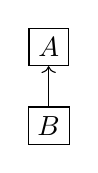
\begin{tikzpicture}
			\node[box] (con) at (0,0) {$A$};
			\node[box] (pre) at (0, -1) {$B$};
			\draw[->] (pre) to (con);
		\end{tikzpicture}
		\figsentence{$A$ because $B$.}
		\caption{Support}
		\label{fig:support}
	\end{subfigure}
	\begin{subfigure}[b]{0.3\textwidth}
		\centering
		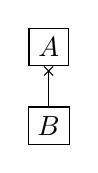
\begin{tikzpicture}
			\node[box] (con) at (0,0) {$A$};
			\node[box] (att) at (0, -1) {$B$};
			\draw[-x] (att) to (con);
		\end{tikzpicture}
		\figsentence{$A$ but $B$.}
		\caption{Attack}
		\label{fig:attack}
	\end{subfigure}
	\begin{subfigure}[b]{0.3\textwidth}
		\centering
		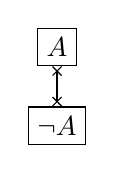
\begin{tikzpicture}
			\node[box] (con) at (0,0) {$A$};
			\node[box] (att) at (0, -1) {$\neg A$};
			\draw[xx] (att) to (con);
		\end{tikzpicture}
		\figsentence{$A$. $\neg A$.}
		\caption{Mutual attack}
		\label{fig:mutual}
	\end{subfigure}
	\caption{Pros and Cons}
	\label{fig:proscons}
\end{figure}


\paragraph{Conjunctions and negation}

\begin{figure}[ht!]
	\centering
	\begin{subfigure}[b]{0.3\textwidth}
		\centering
		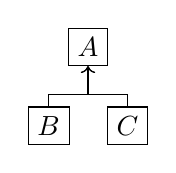
\begin{tikzpicture}
			\node[box] (con) at (0,0) {$A$};
			\node[box] (per1) at (-.5,-1) {$B$};
			\node[box] (per2) at (.5,-1) {$C$};
			\draw[->] (per1) -- ++(0,.4) -| (con);
			\draw[->] (per2) -- ++(0,.4) -| (con);
		\end{tikzpicture}
		\figsentence{$A$ because $B$ and $C$.}
		\caption{Linked/Cooperative support}
		\label{fig:cooperative}
	\end{subfigure}
	\begin{subfigure}[b]{0.3\textwidth}
		\centering
		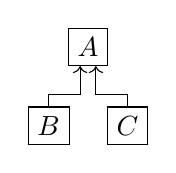
\begin{tikzpicture}
			\node[box] (con) at (0,0) {$A$};
			\node[box] (per1) at (-.5,-1) {$B$};
			\node[box] (per2) at (.5,-1) {$C$};
			\draw[->] (per1) -- ++(0,.4) -| ([xshift=-0.1cm]con.south);
			\draw[->] (per2) -- ++(0,.4) -| ([xshift=0.1cm]con.south);
		\end{tikzpicture}
		\figsentence{$A$ because $B$ and because $C$.}
		\caption{Multiple/Independent support}
		\label{fig:independent}
	\end{subfigure}
	\begin{subfigure}[b]{.3\textwidth}
		\centering
		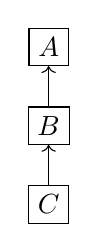
\begin{tikzpicture}
			\node[box] (con) at (0,0) {$A$};
			\node[box] (per1) at (0,-1) {$B$};
			\node[box] (per2) at (0,-2) {$C$};
			\draw[->] (per2) -> (per1);
			\draw[->] (per1) -> (con);
		\end{tikzpicture}
		\figsentence{$A$ because $B$ because $C$.}
		\caption{Chained support/Recursion}
		\label{fig:chained}
	\end{subfigure}
	\caption{Conjunctions}
\end{figure}

Rebuttal only occurs when both $A$ and $\neg A$ occur as premise in the argument, otherwise we drawn them as just an attacking premise. $A$ and $\neg A$ may occur in separate sentences or separate parts of the argument.

Finding out whether $\neg A$ occurs in an argument can be challenging, as for example Tweety being a cat would also imply that Tweety is not a bird. However, for this inference step to take place knowledge about dogs and cats is necessary. (And that is outside the scope of this work for now.)

\paragraph{Recursion}

Only context can be used to disambiguate between these two. We circumvent this by not allowing conjunctions to be the topmost elements of the argument. Each sentence in an argument starts with a conclusion, either followed by pros and cons or not. No a and b at the top.

\paragraph{Rules, warrants, generalizations}

\begin{figure}[ht!]
	\centering
	\begin{subfigure}[b]{0.3\textwidth}
		\centering
		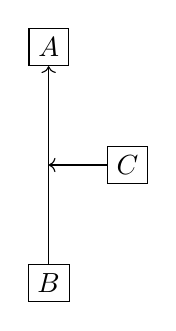
\begin{tikzpicture}
			\node[box] (con) at (0,0) {$A$};
			\node[box] (war) at (1, -1.5) {$C$};
			\node[box] (pre) at (0, -3) {$B$};
			\node[coordinate] (w) at (0, -1.5) {};
			\draw[->] (pre) -- (w) -> (con);
			\draw[->] (war) -> (w);
		\end{tikzpicture}
		\figsentence{$A$ because $B$ and $C_{maj}$.}
		\caption{Warranted support}
		\label{fig:warrantedsupport}
	\end{subfigure}
	\begin{subfigure}[b]{0.3\textwidth}
		\centering
		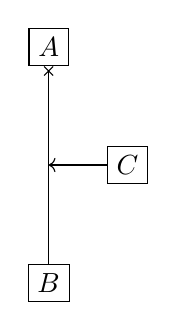
\begin{tikzpicture}
			\node[box] (con) at (0,0) {$A$};
			\node[box] (war) at (1, -1.5) {$C$};
			\node[box] (pre) at (0, -3) {$B$};
			\node[coordinate] (w) at (0, -1.5) {};
			\draw[-x] (pre) -- (w) -> (con);
			\draw[->] (war) -> (w);
		\end{tikzpicture}
		\figsentence{$A$ but $B$ and $C_{maj}$.}
		\caption{Warranted attack}
		\label{fig:warrantedattack}
	\end{subfigure}
	\begin{subfigure}[b]{0.3\textwidth}
		\centering
		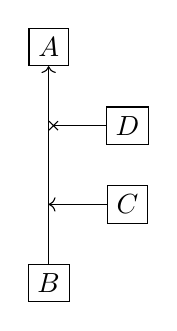
\begin{tikzpicture}
			\node[box] (con) at (0,0) {$A$};
			\node[box] (war) at (1, -2) {$C$};
			\node[box] (pre) at (0, -3) {$B$};
			\node[box] (und) at (1, -1) {$D$};
			\node[coordinate] (u) at (0, -1) {};
			\node[coordinate] (w) at (0, -2) {};
			\draw[->] (pre) -- (w) -- (u) -> (con);
			\draw[->] (war) -> (w);
			\draw[-x] (und) -> (u);
		\end{tikzpicture}
		\figsentence{$A$ because $B$ and $C_{maj}$ but $D$.}
		\caption{Undercutter}
		\label{fig:undercutter}
	\end{subfigure}
	\caption{Support using rules and attack thereof}
\end{figure}

\paragraph{Complications:}

\paragraph{Anaphora resolution}
The premises in the boxes are self-contained: they can not refer to each other using pronouns. In (argumentative) text they can because of the word order, but in a diagram the word order is lost. Therefore we should try to avoid the occurrence of pronouns in the boxes.

\paragraph{Enthymemes}
Parts of the argument are unstated: premises assumed to be known and accepted by all parties are not communicated (or not communicated because they are weak and the speaker does not want to wake sleeping dogs). However, these unstated premises can be supported and attacked. In the diagram, they have to be drawn in order for them to be able to supported or attacked. Hence we need to reconstruct and draw them.

\section{Pros, cons, rules: HASL/0}
HASL/0 is an implementation of the language which focusses on supporting all elements of the argument structure. Combining sentences (or structures) in to larger arguments is done by repeating the premise, not unlike repeating a variable in first-order logic.

\paragraph{Parser} Sentences are tokenized and to each of the tokens a part-of-speech tag (pos-tag) is assigned using spaCy. The tokens are then parsed into argument structures using an Earley parser and the grammar described in this section.

\paragraph{Argument structure} The partial and final argument structures are represented as a graph with nodes and edges, or premises and relations, with a few notable differences: First, a relation can have multiple premises as source to model Cooperative supporting relations between premises (\autoref{fig:cooperative}). Second, a relation can target another relation. This is needed to encode the warranted support relation (\autoref{fig:warrantedsupport}).

\paragraph{Merging claims} At the end of every grammar rule the matched structures are merged. For rules that combine a few words into an \emph{object} this merely involves combining the spans of text into a single span that encompasses both (i.e. `the' + `man' becomes `the man') but when combining sentences the argument structures need to be merged. During this merge premises that were repeated in the text are merged into a single node in the argument graph.

\begin{enumerate}
    \item All premises from both arguments to be merged are added to the list as a pair consisting of the premise id and the premise itself.
    \item Each premise that occurs multiple times in the list is then replaced with the first occurrence.
    \item The list is used to replace all occurrences of the replaced premises with their replacement in the relations.
    \item The resulting set of unique premises and up-to-date relations is used to create a new argument, the result which is yielded after finishing the grammar rule.
\end{enumerate}

\paragraph{Grammar} We start with describing the grammar and parsing process for the basic support and attack relations.

\begin{grammar}
<argument> ::= <premise> `because' <minor-premise> % *> a <~ b

<argument> ::= <premise> `but' <minor-premise> % *> a *~ b
\end{grammar}

\noindent After parsing the rule in a text the argument structure is formed. If we use $a$ and $b$ to denote the text that matched \texttt{<premise>} and \texttt{<minor-premise>} we can describe the argument yielded by matching the first rule as follows: It consists of two premises, $a$ and $b$, and a relation $a <~ b$.

We make the distinction between minor and major premises: minor premises are statements about someone or something particular, e.g. Tweety, Socrates, and `the object' in our examples. Major premises are claims of a more general or generative nature: they are more rule-like and express expectations, for example that birds can fly or that men are mortal.

Minor and major premises we detect in HASL/0 using the following grammar. We use \texttt{<x>} with lower case $x$ to refer to other grammar rules, \texttt{<X>} with upper case $X$ to denote a token that matches one of the part-of-speech tags from \autoref{table:postags}, and \texttt{`x'} to indicate that the token is just the string `x'.

\begin{table}
    \begin{tabular}{lll}
        Tag & Description & Example \\
        \hline
        NN  & noun, singular & bird \\
        NNS & noun, plural & birds \\
        NNP & noun, proper singular & Socrates \\
        MD  & verb, modal auxiliary & can \\
        VBZ & verb, 3rd person singular present \\
        VBP & verb, non-3rd person singular present & are \\
        VBN & verb, past particle & illuminated \\
        DT  & determiner & the, a \\
        JJ  & adjective & red \\
        IN  & preposition & in, on, by \\
        RB  & adverb & not
    \end{tabular}
    \caption{Part-of-speech tags used in HASL, part of the Penn Treebank tag set.}
    \label{table:postags}
\end{table}

\begin{enumerate}
    \item `The man is mortal' and `Socrates is mortal'
    \begin{grammar}
        <minor-premise> ::= <instance> <VBZ> [<RB>] <object>
    \end{grammar}
    \item `Tweety can fly'
    \begin{grammar}
        <minor-premise> ::= <instance> <MD> [<RB>] <VB>
    \end{grammar}

    \item `A man is mortal'
    \begin{grammar}
        <major-premise> ::= <prototype-sg> <VBZ> [<RB>] <object>
    \end{grammar}
    \item `A bird can fly'
    \begin{grammar}
        <major-premise> ::= <prototype-sg> <MD> [<RB>] <VB>
    \end{grammar}
    \item Men are mortal
    \begin{grammar}
        <major-premise> ::= <prototype-pl> <VBP> [<RB>] <object>
    \end{grammar}
    \item Birds can fly
    \begin{grammar}
        <major-premise> ::= <prototype-pl> <MD> [<RB>] <VB>
    \end{grammar}
\end{enumerate}

These rules are supported by definitions for \texttt{object}, \texttt{instance} and the singular and plural versions of \texttt{prototype}. 

Objects are often the objects of sentences:

\begin{enumerate}
    \item `wings' in `Tweety has wings'
    \begin{grammar}
        <object> ::= <NN> \alt <NNS>
    \end{grammar}

    \item `red' in `the object is red'
    \begin{grammar}
        <object> ::= <JJ>
    \end{grammar}

    \item `the object' or `an object'
    \begin{grammar}
        <object> ::= <DT> <NN>
    \end{grammar}

    \item `the red light'
    \begin{grammar}
        <object> ::= <DT> <JJ> <NN>
    \end{grammar}

    \item `illuminated by a red light' for `the light is …'
    \begin{grammar}
        <object> ::= <vbn>

        <vbn> ::= <VBN>
        \alt <VBN> <preposition-phrase>

        <preposition-phrase> ::= <IN> <NNP>
        \alt <IN> <object>
    \end{grammar}
\end{enumerate}

Instances are names, nouns which are preceded by a definite determiner (e.g. `the', `this') and pronouns referring to them such as `he' and `it'.

\begin{grammar}
<instance> ::= <NNP>
\alt <PRP>
\alt <definite-dt> <NN>
\alt <definite-dt> <NNP>

<definite-dt> ::= `the' \alt `this'
\end{grammar}

Prototypes are the indefinite variant of these. Since major premises both often occur as singular and as plural premises we add grammar rules for both. For minor premises we only implement the singular form.

\begin{grammar}
<prototype-sg> ::= <indefinite-dt> <NN>
\alt <indefinite-dt> <NN> <vbn>

<prototype-pl> ::= <NNS>
\alt <NNS> <vbn>

<indefinite-dt> ::= `a'
\end{grammar}

\paragraph{Sentences} Finally, an argumentative text in HASL's language consists of one or more sentences which combine the argument structures into a single argument.

\begin{grammar}
<sentences> ::= <sentences> <sentence>
    \alt <sentence>

<sentence> ::= <argument> `.'
\end{grammar}

\paragraph{Support} The grammar for supporting and attacking premises is incomplete, as it cannot be used to create the cooperative relations. We redefine the support and attack grammar rules to accept one or multiple reasons.

\begin{grammar}
<argument> ::= <premise> `because' <minor-premises> % a <~ b+

<argument> ::= <premise> `but' <minor-premises> % a *~ b+

<minor-premises> ::= <minor-premise>
\alt <minor-premise-list> `and' <minor-premise>

<minor-premise-list> ::= <minor-premise>
\alt <minor-premise-list> `,' <minor-premise>
\end{grammar}

\noindent Using these rules we can already form all argument structures depicted in \autoref{fig:proscons}, either directly or by repeating premises in multiple sentences.

\paragraph{Warranted support and attack} Warranted support and attack combines the usage of the major and minor premise.

\begin{grammar}
<argument> ::= <premise> `because' <minor-premise-list> `and' <major-premise> % (a <~ b+) <~ c

<argument> ::= <premise> `because' <major-premise> `and' <minor-premises> % (a <~ c+) <~ b

<argument> ::= <premise> `but' <minor-premise-list> `and' <major-premise> % (a *~ b+) <~ c

<argument> ::= <premise> `but' <major-premise> `and' <minor-premises> % (a *~ c+) <~ b
\end{grammar}

\noindent These rules effectively add two relations to the argument: one from the minor premises supporting or attacking the conclusion, and one from the major premise supporting the previous relation.

There is no \texttt{major-premise-list} or a way to add multiple major premises to a support relation as we only expect at most one major premise to be relevant per relation.

\paragraph{Undercutter} Lastly we need an extra rule to express the undercutter, as we currently have no way to express an attack on a relation.

\begin{grammar}
<argument> ::= <premise> `because' <minor-premises> `but' <premise> % (a <~ b+) *~ c
\end{grammar}

\paragraph{Result} The resulting grammar is unambiguous: There is only one way for each of the elements of the argument structure to be expressed. For simple examples it is very effective:

\begin{exe}
    \ex Socrates is mortal because he is a man and men are mortal.
    \ex The object is red because the object appears red but it is illuminated by a red light.
\end{exe}

\paragraph{Discussion}
Other structures, such as the chaining or arguments (\autoref{fig:chained}) and two arguments attacking each other (\autoref{fig:mutual}) are verbose to express:

\begin{exe}
    \ex\label{ex:hasl0tbw} Tweety can fly because he is a bird. He is a bird because he has wings.
    \ex\label{ex:hasl0tbnottb} Tweety is a bird but Tweety is not a bird. Tweety is not a bird but Tweety is a bird.
\end{exe}

\noindent Next to that the anaphora in example \ref{ex:hasl0tbw} also occur in the boxes, making the argument more difficult to understand as the order of the sentence, which we normally use to resolve anaphora, is no longer present. If there would be two or more individuals that can be referred to, there is no way to find out to which of these the pronoun referred.

The pronouns also make merging claims more difficult. For examples~\ref{ex:hasl0tbw} and~\ref{ex:hasl0tbnottb} to work the premise needs to be exactly the same. If we would start the second sentence in example~\ref{ex:hasl0tbw} with `Tweety' instead of `He', they would not have been merged into a single box in the argument structure. Having anaphora resolution happen before trying to merge the premises would help this process.


\section{Recursion, anaphora and enthymemes: HASL/1}
paragraph{Recursion}

Because HASL's argumentation scheme allows claims to be both on the sending and receiving end of a support or attack relation at the same time, it is only natural that HASL's language supports nesting arguments as well. This is achieved by allowing the claims that occur in the \texttt{support} and \texttt{attack} rule to be claims with supporting or attacking arguments attached to them.

\begin{grammar}

<claims> ::= <extended-specific-claims>

<extended-specific-claim> ::= <specific-claim> <supports> <attack>

\end{grammar}

\begin{exe}
	\ex\label{ex:c3} Tweety can fly because he is a bird because he has feathers.
\end{exe}

\noindent Example \ref{ex:c3} is a slight alteration of Examples \ref{ex:c1} and \ref{ex:c2} that shows this nesting. Here, Tweety has can fly because he is a bird, but Tweety being bird might be questioned as it needs additional support. This support comes in the form of the claim that Tweety has feathers which, in this argument, supports Tweety being a bird. \autoref{fig:c3} shows the argument as a diagram.

\paragraph{Anaphora resolution}
Pronominal Anaphora resolution---making the connection between `Henry', `the king', and `he', or `Tweety' and `he'---is added to allow one to write more natural sentences without the need of repeating a unique name for each individual in the argument. In the argument diagrams all pronouns are, when possible, rewritten as the name or proper noun of the individual they are referring to, since the argument diagram does not have or maintain the same order of claims, which would make finding out what a pronoun refers to more challenging.

Anaphora resolution is done at every moment partial interpretations are combined, which is when a grammar rule is completely parsed. Each partial interpretation keeps a list of all distinct instances, and for each of these instances a list of occurrences in claims. These lists can be used to identify which current instance is connected to the instance observed in the various claims. The resulting tree-searching algorithm is similar to Hobbs' algorithm \cite{hobbs1978}.

For example, in the sentence `Socrates is mortal because he is a man.', there is only one distinct instance in the final interpretation, namely Socrates. While parsing, both `Socrates' and `he' are observed as instances. So in the final interpretation, the list of observed instances associated with `Socrates' contains both these. By merging these, which in this example happens when the \texttt{expanded-specific-claim} rule finishes, a new instance is created which contains both the name `Socrates' and the pronoun `he'. When drawing the graph, the terminals `Socrates' and `he' can be looked up in the lists and it can be determined that these refer to the same subject. This can then be displayed in the graph (e.g. by associating and printing the same number next to each terminal that refers to this instance).

When merging partial interpretations, if two separate instances are believed to be referring to the same subject, a new canonical instance is created and added to the list with distinct, canonical instances. Then, this new instance is associated with the two merged (previously canonical) instances and all other (non-canonical) instances that were already associated with these two.

For anaphora resolution it is important to know which of the instances came first in the order of the words of a sentence. For example, it is likely that in the sentence `John said he saw a deer.' `he' refers to `John', but in the sentence `He said John saw a deer' `He' is probably not referring to `John'.

\paragraph{Scopes}
The condition claims in rules make use of the \emph{individual} atom in the subject slot of a claim to connect them to each other. To make the sentences readable the noun `something' or `all' is used to name these singular and plural individuals. During the anaphora resolution step this can cause problems, as the `something' from one of these individuals might be linked to the `something' from another one, as would normally happen when individuals repeat the same noun. To counter this individuals inside general claims are assigned a scope, and the scope is limited to the general claim. Individuals with a different scope cannot be merged.

\begin{exe}
	\ex\label{gramscopes} Socrates is mortal because he is a man. Achilles is mortal because he is a man.
	\ex Socrates is mortal because he is a man and because Achilles is mortal because he is a man. (Bit forced example, but shows how `he is a man' is treated as two different premises, even though the words are the same.)
\end{exe}

\paragraph{Enthymeme resolution}
Often, the general claims accepted by HASL/1's grammar can be interpreted as rules, for example in arguments which build upon simple deductive reasoning, like the examples with Tweety and Socrates, but also for example legal language, where an argument consists of multiple conditions which have to be met for a law to be applicable. This structured form of warrants can be used to help with enthymemes: arguments in which the datum or the warrant, or the minor or major clause is left out. In the case of legal rules, it can identify which conditions have been met, and which have not been mentioned.

\begin{exe}
	\ex\label{ex:enthymin} Socrates is mortal because he is a man.
	\ex\label{ex:enthymaj} Socrates is mortal because men are mortal.
\end{exe}

\noindent These sentences are two sentences which respectively the major and minor clause are left out. By looking at the two remaining clauses the missing clause can be reconstructed, or assumed. (The used algorithm is simple, but only appropriate for syllogisms that do not occur often in natural argumentation \cite{saintDizierStede2017}.)

Internally, the conditions of a rule-like major claim are attached to the major claim through a \emph{condition} relation. This type of relation is similar to an attack or support relation, but is only used inside a warrant. This is also done for general claims in the form `All men are mortal', which are represented as, for example, `Something is mortal' with the conditional claim `Something is a man'. As a result, when we have sentence \ref{ex:enthymaj}, generating the assumed specific claim `Socrates is a man' is done based on all condition relations of the general claim `men are mortal', which in this case is only `Something is a man'. The subject, `Socrates', is matched with that of the conclusion and the resulting premise, `Socrates is a man' and the supporting relation is added.

Note that this also works for arguments with warrants with multiple conditions or arguments with multiple claims together supporting the conclusion. In the first case, a minor claim will be constructed for every condition and all these claims together will support the conclusion. In the second case, a condition will be generated for every claim supporting the conclusion via the relation that is missing the major claim.



\section{Evaluation: syllogisms and Toulmin arguments}

\begin{exe}
	\ex Tweety can fly because birds can fly but Tweety is a penguin.

	\ex Harry is a British subject because Harry is a man born in Bermuda but Harry has become naturalized.
\end{exe}

\begin{figure}[ht!]
	\centering
	\begin{subfigure}[b]{\textwidth}
		\centering
		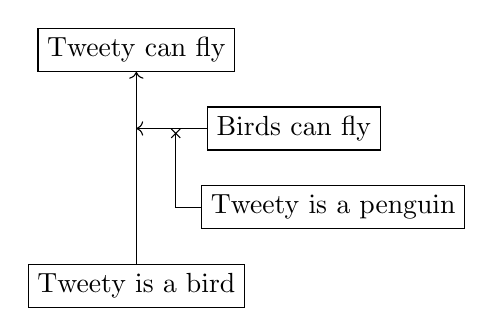
\begin{tikzpicture}
			\node[box] (con) at (0,0) {Tweety can fly};
			\node[box] (min) at (0,-3) {Tweety is a bird};
			\node[box] (maj) at (2,-1) {Birds can fly};
			\node[box] (und) at (2.5,-2) {Tweety is a penguin};
			\node[coordinate] (smaj) at (0,-1) {};
			\node[coordinate] (sund) at (.5,-1) {};
			\node[coordinate] (cund) at (.5,-2) {};
			
			\draw[->] (min) -- (smaj) -| (con);
			\draw[->] (maj) -- (sund) -> (smaj);
			\draw[-x] (und) -- (cund) -> (sund);
		\end{tikzpicture}
		\caption{First interpretation}
	\end{subfigure}

	\begin{subfigure}[b]{\textwidth}
		\centering
		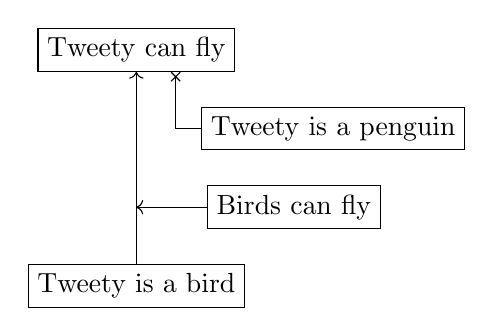
\begin{tikzpicture}
			\node[box] (con) at (0,0) {Tweety can fly};
			\node[box] (min) at (0,-3) {Tweety is a bird};
			\node[box] (maj) at (2,-2) {Birds can fly};
			\node[box] (att) at (2.5,-1) {Tweety is a penguin};
			\node[coordinate] (smaj) at (0,-2) {};
			
			\draw[->] (min) -- (smaj) -| (con);
			\draw[->] (maj) -> (smaj);
			\draw[-x] (att) -| ([xshift=.5cm]con.south);
		\end{tikzpicture}
		\caption{Second interpretation}
	\end{subfigure}
	\figsentence{Tweety can fly because Tweety is a bird and birds can fly but Tweety is a penguin.}
	\caption{Argument diagram from HASL/0}
\end{figure}

\begin{figure}[ht!]
	\centering
	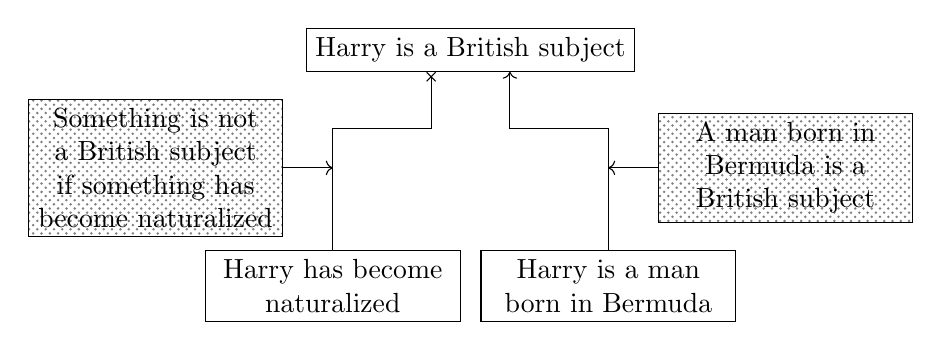
\begin{tikzpicture}
		\node[box] (con) at (0,0) {Harry is a British subject};
		
		\node[box,text width=3cm] (pcon) at (-1.75,-3) {Harry has become naturalized}; % datum
		\node[box,assumed,text width=3cm] (wcon) at (-4,-1.5) {Something is not a British subject if something has become naturalized}; % warrant
		\node[coordinate] (scon) at (-1.75, -1.5) {}; % warrant -> (datum -> concl)
		\node[coordinate] (ccon) at (-1.75, -1) {}; % budge in (datum -> concl) arrow
		
		
		\node[box,text width=3cm] (ppro) at (1.75,-3) {Harry is a man born in Bermuda};
		\node[box,assumed,text width=3cm] (wpro) at (4,-1.5) {A man born in Bermuda is a British subject};
		\node[coordinate] (spro) at (1.75, -1.5) {};
		\node[coordinate] (cpro) at (1.75,-1) {};
		
		\draw[-x] (pcon) -- (scon) -- (ccon) -| ([xshift=-.5cm]con.south);
		\draw[->] (ppro) -- (spro) -- (cpro) -| ([xshift=.5cm]con.south);
		\draw[->] (wcon) -> (scon);
		\draw[->] (wpro) -> (spro);
	\end{tikzpicture}
	\figsentence{Harry is a British subject because Harry is a man born in Bermuda but Harry has become naturalized.}
	\caption{Argument diagram from HASL/1. Shaded boxes are reconstructed major premises.}
\end{figure}


\section{Discussion of related research}

Just adding the assumed missing claims from enthymemes to the argument may not be what the original author of the argument intended. The meaning or weight may become distorted, or it may become clear that the incomplete argument was, after being completed, a bad argument. \cite{waltonReed2005}. 

\begin{table}
	\begin{tabular}{l|ll|}
		& HASL/0 & HASL/1  \\
		\hline
		Support & yes & yes \\
		Attack & yes & yes \\
		Schema recognition & no & via enthymeme resolution \\
		Schema extraction & no & yes
	\end{tabular}
\end{table}

\section{Conclusion}


%
%Diagramming tools (Araucaria, Reason!Able, ArguMed)
%
%Text analysis assistants (Araucaria)
%
%Argument mining
%
%Logical languages (with evaluation)
%
%
%\section{Translating natural language arguments to argument diagrams, and back}
%
%Description of how it all works
%
%(Elementary, representative examples)
%
%\section{Toulmin's diagram}
%
%
%\section{Assessment}
%
%Interesting examples
%
%Things that go wrong!



\bibliographystyle{plain}
\bibliography{cumulative}

\end{document}

